%!TEX TS-program = xelatex

\documentclass {article}

\usepackage{xetexko}
\usepackage[a4paper]{geometry}
\usepackage[usenames,dvipsnames]{xcolor}
\usepackage{mathtools}
\usepackage{amsmath}
\usepackage{fontspec}
\usepackage{hyperref}
\usepackage{graphicx}
\usepackage{listings}
\usepackage{makeidx}
\usepackage{indentfirst}
\usepackage{tikz}
\usetikzlibrary{arrows,automata}


%\setmainfont {NanumMyeongjo}
\setmainfont {UnBatang}
\setmonofont[Scale=0.8]{DejaVu Sans Mono}

\lstdefinestyle{diff}{
  belowcaptionskip=1\baselineskip,
  breaklines=true,
  frame=L,
  xleftmargin=\parindent,
  showstringspaces=false,
  % Diffstart
  morecomment=[f][\color{gray}]{@@},
  % Diffincl
  morecomment=[f][\color{Green}]{+},
  % Diffrem
  morecomment=[f][\color{Red}]{-},
  basicstyle=\footnotesize\ttfamily,
}

\lstdefinestyle{customtxt}{
  belowcaptionskip=1\baselineskip,
  breaklines=true,
  frame=L,
  xleftmargin=\parindent,
  showstringspaces=false,
  basicstyle=\footnotesize\ttfamily,
}

\lstdefinestyle{customc}{
  belowcaptionskip=1\baselineskip,
  breaklines=true,
  frame=L,
  xleftmargin=\parindent,
  language=C,
  showstringspaces=false,
  basicstyle=\footnotesize\ttfamily,
  keywordstyle=\bfseries\color{green!40!black},
  commentstyle=\itshape\color{purple!40!black},
  identifierstyle=\color{blue},
  stringstyle=\color{orange},
}

\lstdefinestyle{customrs}{
  belowcaptionskip=1\baselineskip,
  breaklines=true,
  frame=L,
  xleftmargin=\parindent,
  showstringspaces=false,
  morekeywords={fn,let,mut,pub,use,impl,struct,unsafe,if,for},
  morecomment=[l]{//},
  morecomment=[n]{/*}{*/},
  basicstyle=\footnotesize\ttfamily,
  keywordstyle=\bfseries\color{green!40!black},
  commentstyle=\itshape\color{purple!40!black},
  identifierstyle=\color{blue},
  stringstyle=\color{orange},
}


\begin {document}

\title {Linux kernel 2.6.35 에 시스템 콜 추가}
\input {../../reportauthor.tex}
\maketitle

\section {목적}
\(~~\)리눅스 커널을 패치해서 시스템 콜을 추가하고, 이를 유저 월드에서
호출하는 코드를 작성하고 동작시킴으로서

\vspace{\baselineskip}
\begin {itemize}
  \item 리눅스 커널의 구조를 이해한다.
  \item 시스템 콜이 어떻게 호출되는지를 이해한다.
\end {itemize}

\vspace{\baselineskip}
와 같은 목적을 달성한다.

\section {커널 시스템 콜의 동작}

\(~~\)유저 모드 어플리케이션들은, 커널 월드에서 가능한 작업 (e.g. 하드웨어 제어) 을 수행할 때
자신의 실행을 잠시 중단시키고 커널에 프로그램 진행을 넘기게 된다. 이는 소프트웨어 인터\linebreak
럽트를 통해 이루어지며, 커널은 소프트웨어 인터럽트를 받게 되면, 프로그램의 실행을 유저 모드\linebreak
에서 커널 월드로 전환하게 된다.

리눅스 커널이 시스템 콜 호출을 받게 되면, (INT 0x80) 커널은 유저 모드 프로세스를 중지\linebreak
시키고 커널 월드로 컨트롤을 전환한 뒤  IDT 에서 0x80 항목 - 시스템 콜 핸들링 서브루틴 - system\_call() 을 실행한다.
시스템 콜 핸들링 서브루틴은 sys\_call\_table 에서 시스템 콜 번호를 찾아,
시스템 콜 본체를 실행하게 된다.

시스템 콜 본체가 동작을 종료하면, system\_call() 은 ret\_from\_system\_call() 을 실행해서, 컨트\linebreak
롤을 다시 유저 스페이스로 넘겨주게 된다.\cite {michaeljohnson00}

\section {실제 시스템 콜 추가}
커널에 시스템 콜을 추가할 시에는, 소스 코드의

\vspace{\baselineskip}
\begin {itemize}
  \item arch/x86/include/asm/unistd\_32.h
  \item arch/x86/include/asm/unistd\_64.h
  \item arch/x86/kernel/syscall\_table\_32.S
\end {itemize}

\vspace{\baselineskip}
파일을 수정해, system call 테이블에 추가할 시스템 콜을 넣고

include/linux/syscalls.h
파일에 추가할 system call 의 원형을 정의한 뒤

Makefile 에 추가할 system call 의 코드가 들어있는 디렉토리를 지정하고,
컴파일하면 커널에 새 시스템 콜 엔트리와, 그 시스템 콜이 호출되었을때,
해당 시스템 콜을 실행할 코드가 들어가게 된다.

이제 my\_enqueue, my\_dequeue 가 패치된 커널에서 glibc 의 syscall 호출 함수를 이용해\linebreak
추가한 syscall 번호를 호출하면, System-wide 하게 적용되는
큐의 동작을 확인할 수 있게 된다.

\begin {figure}[h]
  \centering
  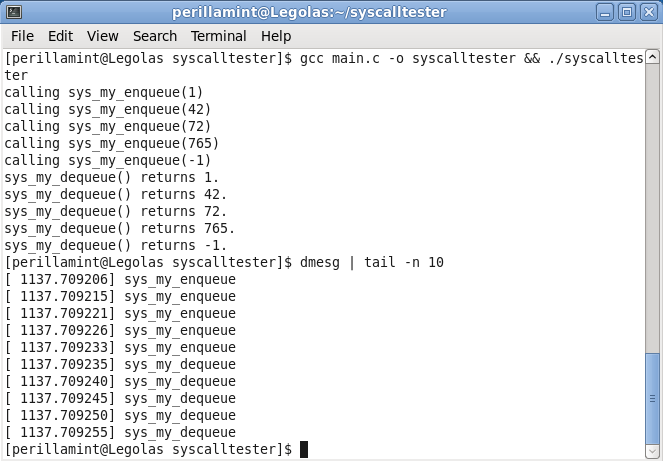
\includegraphics [width=120mm]{syscalluserapp.png}
  \caption {유저 모드 어플리케이션에서 시스템 콜을 부르는 모습.}
  \label{fig:syscalluserapp}
\end {figure}

%\cite [sysdeps/unix/sysv/linux/i386/sysdep.h:196]{mcgrath00}

\section {발생한 문제점}

리눅스 커널의 규모로 인해, 기본적으로 세팅되어있는 커널 설정을 이용해 커널을 빌드할 시 가상\linebreak
화 환경 안에서 사용하지 않을 드라이버를 빌드하는데 상당한 시간이 소요되는 문제가 있었다. 이를 해결하기 위해 Hypervisor 가 에뮬레이션하지 않는다고 확실히 알고 있는 하드웨어에 대한 드라이버 빌드 옵션들을 비활성화해서 커널 빌드에 소요되는 시간을 단축하였다. 

\section {결론}
이 과제를 통해 Linux 의 System call 이 어떻게 동작하는지를 알고, 그것을 사용해서 실제 System call 을 구현할 수 있었다.

% Appendix.
\section {부록 A - 소스 코드}
테스트 환경
Guest OS:\newline
Kernel: Linux 2.6.35.6 AMD64\newline
Distro: Fedora 14\newline
\vspace{\baselineskip}
Host OS:\newline
Kernel: Linux 3.19.0-rc5\newline
Distro: Gentoo linux unstable AMD64\newline
Hypervisor: QEMU version 2.2.1 with KVM.\newline
\vspace{\baselineskip}
Host hardware:\newline
CPU: Intel i7-2670QM\newline

\vspace{\baselineskip}
유저랜드 코드:
\lstinputlisting [style=customc]{syscalltester.c}

\vspace{\baselineskip}
커널 코드 - syscall implementation:

Makefile
\lstinputlisting [style=customtxt]{Makefile-1st-assign}

main.c
\lstinputlisting [style=customc]{main.c}

패치 파일
\lstinputlisting [style=diff]{my_queue_syscall.patch}
\bibliographystyle {plain}
\bibliography {glibc,tldp}
\end {document}
